%%%%%%%%%%%%%%%%%%%%%%%%%%%%%%%%%%%%%%%%%%%%%%%%%%%%%%%%%%%
%% Congratulations, you've made an excellent choice
%% of writing your Tampere University thesis using
%% the LaTeX system. This document attempts to be
%% as complete a template as possible to let you focus
%% on the most important part: the writing itself.
%% Thus the details regarding the visual appearance
%% and even structure have already been worked out
%% for you!
%%
%% I sincerely hope you will find this template useful
%% in completing your thesis project. I've tried to
%% add comments (followed by the % sign) to clarify
%% the structure and purpose of some of the commands.
%% Most of the magic happens in the file tauthesis.cls,
%% which you are more than welcome to take a look at.
%% Just refrain from editing it in the most crucial
%% versions of the thesis!
%%
%% I wish you and your thesis project the best of luck!
%% If this template causes you trouble along the way
%% or if you've any suggestions for improving it,
%% please be in contact through GitHub
%% (<URL HERE>)
%%
%% Yours,
%%
%% Ville Koljonen
%%%%%%%%%%%%%%%%%%%%%%%%%%%%%%%%%%%%%%%%%%%%%%%%%%%%%%%%%%%


\makeatletter

\gdef\@author{Mikhail Shavliuk}
\gdef\@keywords{Data normalization, Transformer models, Deep learning, Machine Learning, Electronic Health Records, Mortality prediction, Time-series forecasting, ECDF, Outliers, Noise robustness}
\gdef\@title{Transformer model for Biomarkers prediction}
\gdef\@subtitle{Evaluating the impact of ECDF normalization on model robustness in clinical data}
\edef\@abstract{This thesis addresses important challenges in predictive analytics in healthcare, specifically focusing on the robustness of machine learning models in the face of outliers and noise within clinical data. Using a transformer-based model and the MIMIC-III dataset, we explore empirical cumulative distribution function (ECDF) normalization as a robust alternative to conventional Z-score normalization. Our findings demonstrate that ECDF normalization significantly enhances model performance, retaining up to 196\% more ROC-AUC for mortality prediction under high uniform noise conditions and reducing mean squared error (MSE) by 31\% for percentile-based forecasting of time-series values, compared to Z-score normalization. These results suggest that ECDF normalization provides a robust approach for predictive analytics in healthcare, reducing the need for manual outlier removal and thus enhancing scalability for larger datasets. In addition to these methodological advances, significant computational optimizations led to a 30x improvement in training speed, which underscores the model's scalability for real-world applications.}
\gdef\@university{Tampere University}

\gdef\@thesistype{Master of Science Thesis}
\gdef\@facultyname{Faculty of Information Technology and Communication Sciences}
\gdef\@examiner{prof. Olli Yli-Harja, prof. Frank Emmert-Streib}
\gdef\@finishyear{2024}
\gdef\@finishmonth{11}
\gdef\@finishday{22}
\gdef\@programmename{Your Programme Name}



\newwrite\file
\immediate\openout\file=\jobname.xmpdata
    \immediate\write\file{\string\Title{\@title}}
    \immediate\write\file{\string\Author{\@author}}
    \immediate\write\file{\string\Keywords{\@keywords}}
    \immediate\write\file{\string\Language{en-US}}
    \immediate\write\file{\string\Subject{\@abstract}}
    \immediate\write\file{\string\PublicationType{thesis}}
    \immediate\write\file{\string\Publisher{\@university}}
    \immediate\write\file{\string\Date{\@finishyear-\@finishmonth-\@finishday}}
\immediate\closeout\file

\makeatother


\pdfminorversion=6
%%%%% PREAMBLE %%%%%

%%%%% Document class declaration.
% The possible optional arguments are
%   finnish - thesis in Finnish (default)
%   english - thesis in English
%   numeric - citations in numeric style (default)
%   authoryear - citations in author-year style
%   apa - citations in APA 7 (available only in English)
%   ieee - citations in IEEE style (available only in English)
%   draft - for faster non-final works, also skips images
%           (recommended, remove in final version)
%   programs - if you wish to display code snippets
% Example: \documentclass[english, authoryear]{tauthesis}
%          thesis in English with author-year citations
\documentclass[ieee]{tauthesis}


\usepackage{siunitx, mhchem, chemfig}
% siunitx: SI units
% mhchem: Chemical formulas
% chemfig: Chemical structures


% The glossaries package throws a warning:
% No language module detected for 'finnish'.
% You can safely ignore this. All other
% warnings should be taken care of!

%%%%% Your packages.
% Before adding packages, see if they can be found
% in tauthesis.cls already. If you're not sure that
% you need a certain package, don't include it in
% the document! This can dramatically reduce
% compilation time.

% Graphs
% \usepackage{pgfplots}
% \pgfplotsset{compat=1.15}

% Subfigures and wrapping text
% \usepackage{subcaption}

% Mathematics packages
\usepackage{amsmath, amssymb, amsthm}
%\usepackage{bm}

% Chemistry packages
% \usepackage{chemfig}
% \usepackage[version=4]{mhchem}

% Text hyperlinking
% \usepackage{hyperref}
% \hypersetup{hidelinks}

% (SI) unit handling
% \usepackage{siunitx}

%\sisetup{
%    detect-all,
%    math-sf=\mathrm,
%    exponent-product=\cdot,
%    output-decimal-marker={,} % for theses in FINNISH!
%}

%%%%% Your commands.

% Print verbatim LaTeX commands
\newcommand{\verbcommand}[1]{\texttt{\textbackslash #1}}

% Basic theorems in Finnish and in English.
% Remove [chapter] if you wish a simply
% running enumeration.
% \newtheorem{lause}{Lause}[chapter]
% \newtheorem{theorem}[lause]{Theorem}

% \newtheorem{apulause}[lause]{Apulause}
% \newtheorem{lemma}[lause]{Lemma}

% Use these versions for individually
% enumerated lemmas
% \newtheorem{apulause}{Apulause}[chapter]
% \newtheorem{lemma}{Lemma}[chapter]

% Definition style
% \theoremstyle{definition}
% \newtheorem{maaritelma}{Määritelmä}[chapter]
% \newtheorem{definition}[maaritelma]{Definition}
% examples in this style

%%%%% Glossary information.

% Use the following lines ONLY if you need more
% than one glossary. The first argument specifies
% a type label for the glossary and the second
% the displayed name.
% \newglossary*{symbs}{Symbols}
% \newglossary{label}{Displayed name}
% ...


%Tools like makeglossaries, bibtex, or biber read these auxiliary files and generate additional
%files (.gls for glossaries, .bbl for bibliographies) that LaTeX will incorporate into the document.

\makeglossaries

% Use this line if using the default glossary.
% Otherwise comment out.
\loadglsentries[main]{tex/glossary}


% Use this line if using more than one glossary.
% Otherwise comment out.
% \loadglsentries[symbs]{tex/sanasto2.tex}

%%%%% Citation information.

% Commonly used bibliography modifications.
% Feel free to play around with them.

%\ExecuteBibliographyOptions{%
%sorting=none,
%maxbibnames=99,
%maxcitenames=2,
%giveninits=true,
%uniquename=init,
%sortcites,
%sortlocale=fin}

%\DefineBibliographyStrings{finnish}{%
%    in = {},
%    pages = {s.},
%    page = {s.}
%}
%\DefineBibliographyStrings{english}{%
%    in = {},
%    pages = {pp.},
%    page = {p.}
%}
%
%\DeclareNameAlias{sortname}{last-first}
%\DeclareNameAlias{author}{last-first}

%\DeclareFieldFormat[%
%    article,inbook,incollection,inproceedings,
%    patent,thesis,unpublished]{citetitle}{#1\isdot}
%\DeclareFieldFormat[%
%    article,inbook,incollection,inproceedings,
%    patent,thesis,unpublished]{title}{#1\isdot}
%\DeclareFieldFormat{pagetotal}{#1 \bibstring{page}}

%\AtBeginBibliography{\renewcommand*{\makelabel}[1]{#1\hss}}

%\DefineBibliographyExtras{english}{\let\finalandcomma=\empty}

\addbibresource{tex/references.bib}

\begin{document}

%%%%% FRONT MATTER %%%%%

\clearpage
\pagenumbering{roman}
\setcounter{page}{0}

%%%%% Thesis information and title page.

% The titles of the work. If there is no subtitle,
% leave the arguments empty. Pass the title in
% the primary language as the first argument
% and its translation to the secondary language
% as the second.


% The examiner information.
% If your work has multiple examiners, replace with
% \examiner[<label>]{<name> \\ <name>}
% where <label> is an appropriate (plural) label,
% e.g. Examiners or Tarkastajat, and <name>s are
% replaced by the examiner names, each on their
% separate line.


% The finishing date of the thesis (YYYY-MM-DD).

% The type of the thesis (e.g. Kandidaatintyö
% or Master of Science Thesis) in the primary
% and the secondary languages of the thesis.

% The faculty and degree programme names in
% the primary and the secondary languages of
% the thesis.

% The keywords to the thesis in the primary and
% the secondary languages of the thesis

\maketitle

%%%%% Abstracts and preface.

% Write the abstract(s) and the preface
% into a separate file for the sake of clarity.
% Pass the appropriate file name as the first
% argument to these commands. Put the \abstract
% in the primary language first and the
% \otherabstract in the secondary language second.
% Those who do not speak Finnish only need the
% first abstract. The second argument of
% the \preface command takes the place where
% the thesis was signed in.
\ifdraftmode\else
    \abstract{tex/abstract.tex}
    \preface{tex/preface.tex}{Tampere}
    %%%%% Table of contents.
    \tableofcontents

    %%%%% Lists of figures, tables, listings and terms.

    % Print the lists of figures and/or tables.
    % Uncomment either of these commands as required.
    % Both are optional, but if there are many important
    % figures/tables, listing them may be a good idea.

    % \listoffigures
    % \listoftables
    % \lstlistoflistings

    % Misc stuff related to how the glossary is displayed.
    % You can especially tweak the lengths to suit you!
    \glsaddall
    \setglossarystyle{taulong}
    \setlength{\glsnamewidth}{0.25\textwidth}
    \setlength{\glsdescwidth}{0.75\textwidth}
    \renewcommand*{\glsgroupskip}{}

    % Print the default glossary of abbreviations,
    % if necessary. Otherwise comment out.
    % The appropriate Finnish variant is 'Lyhenteet'
    \printglossary[title={Glossary}]

    % Print more than one glossary with these lines.
    % Otherwise comment out.
    % \printglossary[type=symbs]
    % \printglossary[type=label]
    % ...

\fi
%%%%% MAIN MATTER %%%%%

\clearpage
\pagenumbering{arabic}
\setcounter{page}{1}


\chapter{Introduction}
\label{ch:introduction}
This document template conforms to the Guide to Writing a Thesis in Tampere University \parencite{thesisguide2018}. A thesis typically includes the following parts:

\begin{enumerate}
    \item[] Title page
    \item[] Abstract in English (and in Finnish)
    \item[] Preface
    \item[] Contents
    \item[] (Lists of figures and tables)
    \item[] List of abbreviations and symbols
    \item Introduction
    \item Theoretical background
    \item Research methodology and material
    \item Results and analysis (possibly in separate chapters)
    \item Conclusions
    \item[] References
    \item[] (Appendices)
\end{enumerate}

Each of these is written as a new \verbcommand{chapter} or using an appropriate command (e.g. \verbcommand{abstract}). Read this document template and its comments carefully. The titles of chapters from 1 to 5 are provided as examples only. You should use more descriptive ones. The title page is created by inserting the relevant information into the commands near the start of the template. The table of contents lists all the numbered headings after it, but not always the preceding headings.

Introduction outlines the purpose and objectives of the presented research. The background information, utilized methods and source material are presented next at a level that is necessary to understand the rest of the text. Then comes the discussion regarding the achieved results, their significance, error sources, deviations from the expected results, and the reliability of your research. The conclusions form the most important chapter. It does not repeat the details already presented, but summarizes them and analyzes their consequences. List of references enables your reader to find the cited sources.

This document is structured as follows. Chapter \ref{ch:esitystyyli} discusses briefly the basics of writing and presentation style regarding the text, figures, tables and mathematical notations. Chapters \ref{ch:viittaustekniikat} and \ref{ch:yhteenveto} summarize the referencing basics and the whole document. Each part also features tips to solving some of the detailed issues that relate to writing in \LaTeX.


\chapter{Writing style}
\label{ch:writing style}
Effective written communication requires both sound content and clear style. Keep the layout of your thesis neat and pay attention to your writing style.

\section{Text}

Do not worry about the layout of the text, this template takes care of it already. Brief basics of writing style:
\begin{itemize}
\item Always think of your reader when you are writing and proceed logically from general to specific.
\item Highlight your key points, for example, by discussing them in a separate \verbcommand{section} or \verbcommand{subsection}, or presenting them in a table or figure. Use italics (\verbcommand{emph}) for emphasis, but don’t overdo it. 
\item Avoid long sentences and complicated statements. A full stop is the best way to end a sentence. 
\item Use active verbs to make a dynamic impression but avoid the first person pronoun I, except in your preface. 
\item Avoid jargon and wordiness. Use established terminology and neutral language.
\item The minimum length of sections and subsections is two paragraphs, and you need to consider the balance of chapters. Paragraphs must always consist of more than one sentence. 
\item Do not use more than three levels of numbered headings, such as 4.4.2. This is covered already by the template.
\item Do not use too many abbreviations. Use capital and small letters consistently.
\end{itemize}

\section{Figures}

You must refer to all the figures in the body text. The reference should preferably appear on the same page as the actual figure or before it. Figures and tables must be numbered consistently and primarily placed at the top of the page, but you are free to decide where they fit best. \LaTeX{} takes care of the numbering, if you specify a unique \verbcommand{label} right after the \verbcommand{caption} of a figure (or a table). Cross-referencing is done by inserting this identifier as the argument to \verbcommand{ref}. Never start (or preferably end) a chapter with a figure, table, equation or list. The caption is placed under the figure.

All figures must be explained in the text body, so that the readers know what they are supposed to notice. Figures generated by analysis software usually need further editing, see Figure \ref{fig:huolittelu} for an example. The figures should be in the same language as other text (even if Figure \ref{fig:huolittelu} violates this recommendation). The recommended font size is the same as that of the body text. The figures must be readable, even if your thesis is printed in greyscale. Whenever possible, use images in vector formats such as \texttt{.eps} or \texttt{.pdf} (\LaTeX{} does not digest \texttt{.svg} files\ldots), as they can be scaled without loss of quality. \LaTeX{} itself also comes with powerful packages for drawing vector graphics (\texttt{tikz}) \parencite{tikz} and graphs (\texttt{pgfplots}) \parencite{pgfplots}. Figure pgf-example shows an example of a graph generated using the latter.

\begin{figure}
\centering
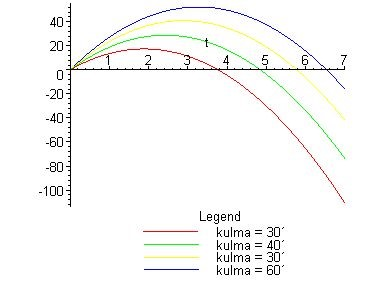
\includegraphics[width=\textwidth]{figures/bad-example}
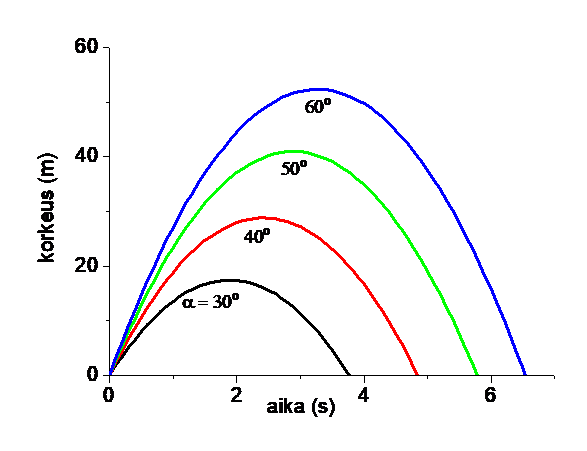
\includegraphics[width=\textwidth]{figures/good-example}
\caption[This is a short caption.]{Diagrams should be edited before publication. The diagram on the right is an edited version of the one on the left.}
\label{fig:huolittelu}
\end{figure}

\section{Tables}

Taulukot sopivat hyvin erityisesti numeerisen informaation esittämiseen tiiviissä muodossa. Kuvien tapaan taulukot numeroidaan ja varustetaan otsikolla, kuten taulukossa. Taulukkoteksti sijoitetaan samalle sivulle taulukon kanssa ja taulukon yläpuolelle. Suureet, lyhenteet ja symbolit selitetään tarvittaessa tekstissä. Kaikkiin taulukoihin on viitattava tekstissä, mieluummin ennen taulukkoa. Taulukon keskeinen sanoma ja tulkintaohjeet selitetään tekstissä.

Taulukon sarakkeet otsikoidaan, ja suureet sekä yksiköt laitetaan näkyviin. Jos otsikkoriviä tarvitsee erottaa muusta taulukosta, tee se korostamalla (\verbcommand{emph}). Taulukon järjestyksellä on suuri merkitys. Jokaista solua ei pidä ympäröidä reunaviivalla, koska taulukosta tulee raskaslukuinen. Lisää vaakaviiva taulukon ylä- ja alareunaan. Vaakaviivoja voi käyttää esimerkiksi 4--5 rivin välein, ellei tietoja muuten ole jaettu kategorioihin tai selkeys sitä vaadi. Sarakkeen numeroarvot tasataan desimaalipilkun kohdalta, jolloin arvoja on helppo vertailla. Tämä tapahtuu \LaTeX{}issa helposti \texttt{siunitx}-paketin \parencite{siunitx} taulukkomateriaalin avulla. Tavoitteena on, että suureet ilmaistaan SI-yksikössä ja käytetään joko vakiintuneita etuliitteitä tai kymmenen potenssin muotoja siten, että ne voidaan laittaa otsikkoriville (katso tässäkin \texttt{siunitx}). Muutamia suosituksia taulukoiden ja kuvien käytöstä löydät lähteestä \parencite{pubadvice2009}.

Tables are convenient for presenting information in a concise way, especially numerical data. Tables have numbered captions, see Table \ref{tab:taulukkoesimerkki} for an example. The caption is placed on the same page but above the table, unlike the captions that accompany figures. You must refer to all the tables in the body text. In addition, you must discuss the content of any tables in the body text to ensure that readers understand their relevance.

Mark the titles of the columns and units clearly. You can use \verbcommand{emph} to highlight the titles, if necessary. The order of the columns and rows must be carefully considered. Do not surround all the cells with a border, as it may make your table harder to read. Put a line on top and bottom of the table. You can add a horizontal line between every 4–5 rows, if the data is not grouped into categories. The numbers are aligned at the decimal point for easy comparison. This is easily done in \LaTeX{} using the tabular material from the \texttt{siunitx} package \parencite{siunitx}. You should preferably use SI units, established prefixes and rewrite large numbers so that the power of ten should be placed in the title of the column instead of each row, if possible. More suggestions can be found in \parencite{pubadvice2009}.


\section{Mathematical notation and equations}

Numbers are generally written using numerals for the sake of clarity, for example ``6 stages'' rather than ``six stages'', which is nevertheless strongly preferred to ``a couple of stages''. You should also use a thousand separator, i.e. instead of 55700125. Never omit the leading zero in decimals. A comma is used as a decimal separator in the Finnish language and a period in the English language. These details are covered by this template and the \texttt{siunitx} package \parencite{siunitx}, if allowed to do so.

Like numbers, it is advisable to abbreviate units of measurement. There is a space between the number and the unit, but you must keep them on the same line. The space is somewhat shorter than a word space, see 1.0 \si{\micro\metre} and \SI{1.0}{\micro\metre} for comparison. It is better to compile a table or graph than include a great deal of numerical values in the body text. Use precise language and put numbers on a scale (small, fast, expensive).

Use generally known and well defined concepts and standard conventions and symbols for representing them. New concepts should be defined when they appear in the text for the first time. Upper case and lower case letters mean different things in symbols and units of measurement. Do not use the same symbol to mean different things.

Strings of mathematical symbols such as $\Theta(n^2)$ are typeset in \LaTeX{} using the math mode. Simple formulas may be displayed within the body of the text without numbering. As an example of a highlighted formula, the Newton’s Second Law of Motion can be written in the following way:
\begin{equation}\label{eq:newtonsecondlaw}
    m\mathbf{a} = \mathbf{F},
\end{equation}
where $m$ denotes the mass of an object, $\mathbf{a}$ its acceleration, and $\mathbf{F}$ the net force it experiences. Please note that all the variables must be defined at the point of their first appearance. The formulae are shown in a different typeface on purpose and the symbols are almost always italicised. Vectors can be written in boldface as above (the convention in printed material) or with an arrow, such as $\vec{v}$. Dimensional numbers can be written using the \verbcommand{SI} command:
\begin{equation*}
    \Vert\mathbf{F}\Vert = m\Vert\mathbf{a}\Vert = \SI{10}{\kilogram} \cdot \SI{9.81}{\metre\per\second\squared} = \SI{98.1}{\newton}.
\end{equation*}

Mathematical formulae are numbered, if they are written on separate lines and referred to in the main body of the text. The number is usually put in parenthesis and right aligned, see equation \eqref{eq:newtonsecondlaw} for an example. Include any punctuation (commas, periods) surrounding an equation in the equations themselves, such as shown in \eqref{eq:newtonsecondlaw}. Occasionally the elements of mathematical text are preceded by an identifier, such as Definition 1 or Theorem 1 \parencite{matohje2009}.

Do not start a sentence with a mathematical symbol but add some word, such as the name or type of the symbol in front of it. Variables, such as $x$ and $y$, are generally presented in italics, whereas elementary functions, special functions and operators are not: $\sin(2x + y)$ or
\begin{equation*}
    \lim_{x \rightarrow -1}\frac{x^2 - 1}{x + 1} = -2.
\end{equation*}
As a rule of thumb, it is best to rely on the automated formatting of an equation editor, such as the one provided by \LaTeX{} \parencite{notsoshort}.

Even those requiring different chemical symbols are not left without support by the \LaTeX{} system. Molecular formulae and stoichiometric equations, such as \ce{CH3CH2CH2COOH} and
\begin{center}
    \ce{N2 (g) + 3 H2 (g) <=> 2 NH3 (g)}
\end{center}


There is a learning curve to writing these elements, especially the structural formulae, but it is good to know that there are ways of accomplishing them.

\section{Programs and algorithms}

Codes and algorithms are written using a \texttt{monospaced font}. If the length of the code or algorithm is less than 10 lines and you do not refer to it later on in the text, you can present it similarly to formulas. If the code is longer but shorter than a page, you present like a figure (see Program \ref{prog:esimerkki}) titled ``Program'' or ``Algorithm''. See the typesetting commands in this template for a method of setting the name manually.

You should add some comments to the code and indent it consistently. The actions performed by the code must be outlined in broad terms in the body text. Line numbers make it much easier to refer to the code in the text. \LaTeX{} includes a package called \texttt{listings} \parencite{listings,notsoshort}, which can handle code very conveniently, include real code files, add row numbers, and highlight the reserved words. Use this for any code representation in \LaTeX.


\section{Accessible thesis}

The Finnish law, following the European Union directive 2016/2102 on accessibility of the websites and mobile applications of public sector bodies, demands that any electronic publications are made appropriately accessible (within reason). This also applies to your thesis, and therefore you should know or find out what is expected of you and your work. The writer or maintainer of the template assumes no responsibility on behalf of thesis authors!

This template aims to help as much as possible with improving the accessibility of the final document. Unfortunately, as of 2021 (and most likely up to 2024), the \LaTeX{} system is incapable of producing PDF files that would conform to the accessible PDF/UA standard, or even the slightly less demanding university guidelines. The main issue is that \LaTeX{} carefully throws away much of the needed structural information as soon as possible to save memory (which was a real issue back in the 80's and 90's). This does not mean that all is lost, and you should still strive for maximum accessibility!

As with the required styles in theses, this template tries to take care of many things automatically for you. The few things you do need to take into account while writing are
\begin{enumerate}
\item the language you use is clear and unambiguous, and that nothing essential is conveyed through visual formatting only,
\item alternative texts (or alt texts) for \emph{all} images you include in the thesis,
\item required document metadata that include the title and the main language of your work,
\item compatibility of mathematics environment with the automated alt text solution.
\end{enumerate}
The instructions for addressing these are as follows.
\begin{enumerate}
\item Do as was described. Use external services for assessing the easy-to-read nature of your text, if necessary.
\item Use the command \texttt{\textbackslash pdftooltip\{\ldots\}\{\ldots\}} from the \texttt{pdfcomment} package (included automatically).
\begin{verbatim}
\begin{figure}
\pdftooltip{\includegraphics[...]{...}}%
{Figure. This alternative text describes
what seeing users see in the image.}
\caption{Figure caption}
\label{fig:somelabel}
\end{figure}
\end{verbatim}
Notice that the caption and the alternative text of an image serve entirely different purposes, and there for the alt text should never be just a copy of the caption! (Also screen readers will always read the caption in addition to the alt text.) Be verbose in the alt texts, but try to focus on the most essential meanings conveyed by the image.
\item Always keep the document metadata fields in the pre-preamble of \texttt{main.tex} up-to-date.
\item Never use the old \TeX{} style \verb+$...$+ and \verb+$$...$$+ environments for math, and instead use the \LaTeX{} style \verb+\(...\)+ and \verb+\[...\]+. The double dollar display math should never be used anyway.

Most of the math environments from \texttt{amsmath}, such as \texttt{equation}, \texttt{equation*} and \texttt{align}, are fine to use and get correct alt texts automatically. In contrast, no math environment from a package other than \texttt{amsmath} is supported! The alternative text for all mathematics environments is the \LaTeX{} source code, until a better solution arrives.
\end{enumerate}



\chapter{Referencing styles}
\label{ch:referencing styles}
Different referencing styles determine how you create in-text citations and the bibliography (list of references). Two common referencing styles are presented in this chapter:
\begin{enumerate}
    \item Numeric referencing (Vancouver system), such as [1], [2], \ldots
    \item Name-year (Harvard) system, such as (Weber 2001), (Kaunisto 2003), \ldots
\end{enumerate}
A numeric reference is inserted in square brackets, whereas the last name of the author and the year of publication are given in parentheses. Both styles are acceptable, but the conventions for referencing vary between disciplines. You must pick one and use is consistently throughout your thesis.

The most commonly used tool for creating bibliographies in \LaTeX{} is the Bib\TeX. It is, however, old already, and the Bib\LaTeX{} \parencite{biblatex} is a more flexible and powerful system to replace it. In practice, most of the scientific publishing relies on the deprecated tool, but a change is at hand. For these reasons, this template guides towards using Bib\LaTeX.

Both of the mentioned systems are based on gathering the bibliographic information from the sources to a \texttt{.bib} file using a specialised syntax. The program reads both this file and the document being written, and then forms the references and the bibliography based on this information. The following contains instructions for using both citation styles with Bib\LaTeX. This template defaults to the use of the numeric system, and this can be reverted to the other style by adding \texttt{authoryear} as an optional argument to the document class.

\section{In-text citations}

In-text citations are placed within the body of the text as close to the actual citation as possible. The citation is generally placed within the sentence before the next period.

\begin{quotation}
\noindent Weber argues that\ldots [1].

\noindent Cattaneo et al. introduce in their study [2] a new\ldots

\noindent The result is\ldots [1, p. 23]. One must also note\ldots [1, pp. 33--36]

\noindent In accordance with the presented theory\ldots (Weber 2001).

\noindent It must especially be noted\ldots (Cattaneo et al. 2004).

\noindent Weber (2001, p. 230) has stated\ldots

\noindent Based on literature in the field [1, 3, 5]\ldots

\noindent Based on literature in the field [1][3][5]\ldots

\noindent The topic has been widely studied [6--18]\ldots

\noindent\ldots existing literature (Weber 2001; Kaunisto 2003; Cattaneo et al. 2004) has\ldots
\end{quotation}

Each of the sources listed in the \texttt{.bib} file must be associated with a unique identifier at the beginning of the entry. These identifiers should be chosen as descriptively as possible, since all citations are created using them. In the numeric system each citation is typeset using the \verbcommand{cite} command, for example \verbcommand{cite\{notsoshort\}}. This produces \cite{notsoshort}, for instance, depending on the final list of references. Additional information can be introduced using the optional arguments: writing \verbcommand{cite[p. 30]\{notsoshort\}} produces \cite[p. 30]{notsoshort} and \verbcommand{cite[see][p. 30]\{notsoshort\}} results in \cite[see][p. 30]{notsoshort}.

The name-year system is more complicated simply because of the greater number of options available, as seen above. The Bib\LaTeX{} logic remains the same, however, the commands change. The most important commands are \verbcommand{parencite}, \verbcommand{parencite*}, \verbcommand{citeauthor} and \verbcommand{textcite}, which produce (Oetiker et al. 2018), (2018), Oetiker et al. and Oetiker et al. (2018), respectively. More commands can be found in the documentation \parencite{biblatex}.

\section{List of references}

At least the
\begin{itemize}
    \item author(s),
    \item title,
    \item time of publication,
    \item publisher,
    \item pages (books and journals), and
    \item website URL
\end{itemize}
are provided per source as bibliographic information, if known. The Bib\LaTeX{} takes care of presenting them in an internally consistent manner. When using this system it is imperative to know the type of the source: a journal article, a book, conference proceedings, a report and a patent are only examples of the various possibilities. This information is also included in the \texttt{.bib} file, and the presentation is automatically taken care of based on the type of the source. Below there is an example of the syntax and information needed in the \texttt{.bib} file for citing a journal article.

\texttt{
\begin{quotation}
    \noindent @article\{braams1991babel,\\
    title=\{Babel, a multilingual style-option system \\
    for use with \textbackslash LaTeX’s standard document styles\},\\
    author=\{Braams, Johannes L\},\\
    journal=\{TUGboat\},\\
    volume=\{12\},\\
    number=\{2\},\\
    pages=\{291--301\},\\
    year=\{1991\}\\
    \}
\end{quotation}
}

The above shows as
\begin{enumerate}[label={[\arabic*]}]
    \item J. L. Braams. Babel, a multilingual style-option system for use with \LaTeX's standard document styles. \emph{TUGboat} 12.2 (1991), 291--301.
    \item[] Braams, J. L. (1991). Babel, a multilingual style-option system for use with \LaTeX's standard document styles. \emph{TUGboat} 12.2, 291--301.
\end{enumerate}
in the different citation styles. It is preferable to order the list of references alphabetically by the first author's last name. This template conforms automatically to this convention. An excellent way for the easy formation of citation entries is to find a template using Google Scholar. It produces a good first try for the use of Bib\TeX{} and Bib\LaTeX{}. In addition to the documentation, \parencite{bibmanagement} provides a good summary of the different citation types and their associated fields.

\chapter{Conclusion}
\label{ch:conclusion}
This template and the writing guidelines should help achieving a consistently formatted and clear documents. A similar template is also available for Word.

Every writing and presentation must have a conclusion. This fact is here emphasized by having this short and rather artificial summary also in this template. A concise summary table can be a good way for providing an overview of the most important points.

Lastly, some final points regarding this template. To prepare the document, use the pdf\LaTeX{} compiler. This option is quite easily found in most \LaTeX{} editors, and when using the terminal simply choose \texttt{pdflatex} as the command. The (list of) references is created using the biber program, found similarly. To typeset the list of abbreviations and symbols requires a run of makeindex on the document. If it seems like the table of contents or the cross-references do not display correctly, try compiling the document again using pdf\LaTeX{}. Finally, if you run into errors while compiling, make sure that your \TeX{} distribution is up to date.

The template has been developed in the Overleaf environment, and the author warmly recommends the usage of its version 2 in writing theses. The easiest way to gain access to the document template is to ask for a copy link to the project from the supervisor of the work, or from the maintainer of this template. To use Overleaf, however, requires a user account and constant access to the Internet.

Hopefully, an up-to-date version of the template is also available in the university intranet. The template has been tested and found to work in the Windows system Mik\TeX{} and the Unix-based system \TeX{} Live environments. The first of these can automatically install the possibly missing packages, but with the latter you may have to install them, or up-to-date versions of them manually.


\ifdraftmode\else
    %%%%% Bibliography/references.

    % Print the bibliography according to the
    % information in ./tex/references.bib and
    % the in-line citations used in the body of
    % the thesis.
    % \emergencystretch=2em
    \printbibliography[heading=bibintoc]
\fi

%%%%% Appendices.

% Use only if it clarifies the structure of
% the document. Remember to introduce each
% appendix and its content.

    \begin{appendices}

        \chapter{Sample attachment}
        \label{ch:appendix}
        Lorem ipsum dolor sit amet, consectetur adipiscing elit, sed do eiusmod
tempor incididunt ut labore et dolore magna aliqua. Sed risus pretium
quam vulputate dignissim suspendisse in est. Feugiat scelerisque varius
morbi enim. Enim sit amet venenatis urna cursus eget nunc. Vel fringilla
 est ullamcorper eget. Dolor sit amet consectetur adipiscing elit ut.
Eget egestas purus viverra accumsan in nisl nisi scelerisque. Tortor
consequat id porta nibh venenatis cras sed felis. Maecenas sed enim ut
sem viverra aliquet. Sed viverra tellus in hac habitasse platea
dictumst. A diam sollicitudin tempor id eu nisl. A arcu cursus vitae
congue mauris. Eget mi proin sed libero. Purus gravida quis blandit
turpis cursus. Tellus rutrum tellus pellentesque eu tincidunt tortor.
Euismod in pellentesque massa placerat. Tempus quam pellentesque nec nam
 aliquam sem et. Vestibulum sed arcu non odio euismod lacinia at quis
risus. Aliquam vestibulum morbi blandit cursus. Feugiat vivamus at augue
 eget arcu.
Lorem
 ipsum dolor sit amet, consectetur adipiscing elit, sed do eiusmod
tempor incididunt ut labore et dolore magna aliqua. Sed risus pretium
quam vulputate dignissim suspendisse in est. Feugiat scelerisque varius
morbi enim. Enim sit amet venenatis urna cursus eget nunc. Vel fringilla
 est ullamcorper eget. Dolor sit amet consectetur adipiscing elit ut.
Eget egestas purus viverra accumsan in nisl nisi scelerisque. Tortor
consequat id porta nibh venenatis cras sed felis. Maecenas sed enim ut
sem viverra aliquet. Sed viverra tellus in hac habitasse platea
dictumst. A diam sollicitudin tempor id eu nisl. A arcu cursus vitae
congue mauris. Eget mi proin sed libero. Purus gravida quis blandit
turpis cursus. Tellus rutrum tellus pellentesque eu tincidunt tortor.
Euismod in pellentesque massa placerat. Tempus quam pellentesque nec nam
 aliquam sem et. Vestibulum sed arcu non odio euismod lacinia at quis
risus. Aliquam vestibulum morbi blandit cursus. Feugiat vivamus at augue
 eget arcu.
Lorem
 ipsum dolor sit amet, consectetur adipiscing elit, sed do eiusmod
tempor incididunt ut labore et dolore magna aliqua. Sed risus pretium
quam vulputate dignissim suspendisse in est. Feugiat scelerisque varius
morbi enim. Enim sit amet venenatis urna cursus eget nunc. Vel fringilla
 est ullamcorper eget. Dolor sit amet consectetur adipiscing elit ut.
Eget egestas purus viverra accumsan in nisl nisi scelerisque. Tortor
consequat id porta nibh venenatis cras sed felis. Maecenas sed enim ut
sem viverra aliquet. Sed viverra tellus in hac habitasse platea
dictumst. A diam sollicitudin tempor id eu nisl. A arcu cursus vitae
congue mauris. Eget mi proin sed libero. Purus gravida quis blandit
turpis cursus. Tellus rutrum tellus pellentesque eu tincidunt tortor.
Euismod in pellentesque massa placerat. Tempus quam pellentesque nec nam
 aliquam sem et. Vestibulum sed arcu non odio euismod lacinia at quis
risus. Aliquam vestibulum morbi blandit cursus. Feugiat vivamus at augue
 eget arcu.Lorem ipsum dolor sit amet, consectetur adipiscing elit, sed do eiusmod
tempor incididunt ut labore et dolore magna aliqua. Sed risus pretium
quam vulputate dignissim suspendisse in est. Feugiat scelerisque varius
morbi enim. Enim sit amet venenatis urna cursus eget nunc. Vel fringilla
 est ullamcorper eget. Dolor sit amet consectetur adipiscing elit ut.
Eget egestas purus viverra accumsan in nisl nisi scelerisque. Tortor
consequat id porta nibh venenatis cras sed felis. Maecenas sed enim ut
sem viverra aliquet. Sed viverra tellus in hac habitasse platea
dictumst. A diam sollicitudin tempor id eu nisl. A arcu cursus vitae
congue mauris. Eget mi proin sed libero. Purus gravida quis blandit
turpis cursus. Tellus rutrum tellus pellentesque eu tincidunt tortor.
Euismod in pellentesque massa placerat. Tempus quam pellentesque nec nam
 aliquam sem et. Vestibulum sed arcu non odio euismod lacinia at quis
risus. Aliquam vestibulum morbi blandit cursus. Feugiat vivamus at augue
 eget arcu.
Lorem
 ipsum dolor sit amet, consectetur adipiscing elit, sed do eiusmod
tempor incididunt ut labore et dolore magna aliqua. Sed risus pretium
quam vulputate dignissim suspendisse in est. Feugiat scelerisque varius
morbi enim. Enim sit amet venenatis urna cursus eget nunc. Vel fringilla
 est ullamcorper eget. Dolor sit amet consectetur adipiscing elit ut.
Eget egestas purus viverra accumsan in nisl nisi scelerisque. Tortor
consequat id porta nibh venenatis cras sed felis. Maecenas sed enim ut
sem viverra aliquet. Sed viverra tellus in hac habitasse platea
dictumst. A diam sollicitudin tempor id eu nisl. A arcu cursus vitae
congue mauris. Eget mi proin sed libero. Purus gravida quis blandit
turpis cursus. Tellus rutrum tellus pellentesque eu tincidunt tortor.
Euismod in pellentesque massa placerat. Tempus quam pellentesque nec nam
 aliquam sem et. Vestibulum sed arcu non odio euismod lacinia at quis
risus. Aliquam vestibulum morbi blandit cursus. Feugiat vivamus at augue
 eget arcu.
Lorem
 ipsum dolor sit amet, consectetur adipiscing elit, sed do eiusmod
tempor incididunt ut labore et dolore magna aliqua. Sed risus pretium
quam vulputate dignissim suspendisse in est. Feugiat scelerisque varius
morbi enim. Enim sit amet venenatis urna cursus eget nunc. Vel fringilla
 est ullamcorper eget. Dolor sit amet consectetur adipiscing elit ut.
Eget egestas purus viverra accumsan in nisl nisi scelerisque. Tortor
consequat id porta nibh venenatis cras sed felis. Maecenas sed enim ut
sem viverra aliquet. Sed viverra tellus in hac habitasse platea
dictumst. A diam sollicitudin tempor id eu nisl. A arcu cursus vitae
congue mauris. Eget mi proin sed libero. Purus gravida quis blandit
turpis cursus. Tellus rutrum tellus pellentesque eu tincidunt tortor.
Euismod in pellentesque massa placerat. Tempus quam pellentesque nec nam
 aliquam sem et. Vestibulum sed arcu non odio euismod lacinia at quis
risus. Aliquam vestibulum morbi blandit cursus. Feugiat vivamus at augue
 eget arcu.
Lorem
 ipsum dolor sit amet, consectetur adipiscing elit, sed do eiusmod
tempor incididunt ut labore et dolore magna aliqua. Sed risus pretium
quam vulputate dignissim suspendisse in est. Feugiat scelerisque varius
morbi enim. Enim sit amet venenatis urna cursus eget nunc. Vel fringilla
 est ullamcorper eget. Dolor sit amet consectetur adipiscing elit ut.
Eget egestas purus viverra accumsan in nisl nisi scelerisque. Tortor
consequat id porta nibh venenatis cras sed felis. Maecenas sed enim ut
sem viverra aliquet. Sed viverra tellus in hac habitasse platea
dictumst. A diam sollicitudin tempor id eu nisl. A arcu cursus vitae
congue mauris. Eget mi proin sed libero. Purus gravida quis blandit
turpis cursus. Tellus rutrum tellus pellentesque eu tincidunt tortor.
Euismod in pellentesque massa placerat. Tempus quam pellentesque nec nam
 aliquam sem et. Vestibulum sed arcu non odio euismod lacinia at quis
risus. Aliquam vestibulum morbi blandit cursus. Feugiat vivamus at augue
 eget arcu.
Lorem
 ipsum dolor sit amet, consectetur adipiscing elit, sed do eiusmod
tempor incididunt ut labore et dolore magna aliqua. Sed risus pretium
quam vulputate dignissim suspendisse in est. Feugiat scelerisque varius
morbi enim. Enim sit amet venenatis urna cursus eget nunc. Vel fringilla
 est ullamcorper eget. Dolor sit amet consectetur adipiscing elit ut.
Eget egestas purus viverra accumsan in nisl nisi scelerisque. Tortor
consequat id porta nibh venenatis cras sed felis. Maecenas sed enim ut
sem viverra aliquet. Sed viverra tellus in hac habitasse platea
dictumst. A diam sollicitudin tempor id eu nisl. A arcu cursus vitae
congue mauris. Eget mi proin sed libero. Purus gravida quis blandit
turpis cursus. Tellus rutrum tellus pellentesque eu tincidunt tortor.
Euismod in pellentesque massa placerat. Tempus quam pellentesque nec nam
 aliquam sem et. Vestibulum sed arcu non odio euismod lacinia at quis
risus. Aliquam vestibulum morbi blandit cursus. Feugiat vivamus at augue
 eget arcu.


    \end{appendices}

\end{document}
